\section{Data and Methods}
\label{sec:data_methods}

This section details the datasets, mathematical formulations, architectural models, and algorithmic extensions constituting the NeuroTensor framework.

\subsection{Multimodal Datasets and Problem Formulations}
\label{subsec:datasets}
To evaluate the flexibility of low-rank deep tensor models, we examine four distinct multimodal datasets spanning hyperspectral imaging, facial photometry, video compressive sensing, and dynamic tomography (Table~\ref{tab:dataset_specs}).

\begin{table}[htbp]
\centering
\caption{Benchmark Multimodal Dataset Specifications and Inverse Problem Configurations.}
\label{tab:dataset_specs}
\begin{adjustbox}{width=0.98\textwidth}
\begin{tabular}{lcccccc}
\toprule
\textbf{Dataset} & \textbf{Physical Modality} & \textbf{Dimensions} & \textbf{Total Voxels} & \textbf{Rank $R$} & \textbf{Factorization Type} & \textbf{Observation Task} \\
\midrule
\textbf{ICVL Benchmark} & Hyperspectral Image & $174 \times 164 \times 260$ & $7,419,360$ & $20$ & 2-Factor: $\mathbf{U} \mathbf{V}^T$ & Mixed Poisson--Gaussian Denoising \\
\textbf{Yale Face B} & Photometric Facial Tensor & $192 \times 168 \times 64$ & $2,064,384$ & $20$ & 3-Way CP: $\llbracket \mathbf{U}, \mathbf{V}, \mathbf{W} \rrbracket$ & 3D Volumetric Tensor Denoising \\
\textbf{Video CS} & Compressive Video Frames & $32 \times 32 \times 16$ & $16,384$ & $8$ & 3-Way CP: $\llbracket \mathbf{U}, \mathbf{V}, \mathbf{W} \rrbracket$ & Compressive Sensing Reconstruction \\
\textbf{PET/CT Volume} & Dynamic Clinical Tomogram & $128 \times 128 \times 56$ & $917,504$ & $16$ & 3-Way CP: $\llbracket \mathbf{U}, \mathbf{V}, \mathbf{W} \rrbracket$ & Sparse-View Projection Recovery \\
\bottomrule
\end{tabular}
\end{adjustbox}
\end{table}

\textbf{ICVL Hyperspectral Benchmark:} The primary benchmark comprises $174 \times 164$ spatial pixels across $260$ contiguous spectral bands ($400\text{--}700\text{ nm}$) \citep{arad2016sparse}, normalized to $[0, 1]$. Degradation follows a mixed Poisson--Gaussian noise model:
\begin{equation}
\label{eq:noise_model}
Y^\text{noisy}(h, w, b) = \frac{\mathcal{P}\big(Y^\text{clean}(h, w, b) \cdot \tau\big)}{\tau} + \mathcal{N}\big(0, \sigma^2\big)
\end{equation}
with photon arrival rate $\tau = 100$ and thermal readout noise $\sigma = 0.046$, establishing an input PSNR of approximately $28.43\text{ dB}$.

\textbf{Volumetric Datasets:} Cross-application evaluation incorporates: (1) \textit{Extended Yale Face B} ($192 \times 168 \times 64$) under varying illumination angles; (2) \textit{Video Compressive Sensing} ($32 \times 32 \times 16$) reconstructed from coded-aperture projections; and (3) \textit{Dynamic PET/CT} ($128 \times 128 \times 56$) evaluating cross-slice radioactive tracer continuity.

\subsection{Theoretical Foundations of DeepTensor}
\label{subsec:deeptensor_foundations}
In the 2-factor hyperspectral model, the matricized tensor $Y_{(1)} \in \mathbb{R}^{HW \times B}$ is factored into spatial and spectral factor matrices:
\begin{equation}
\hat{Y}_{(1)} = \mathbf{U} \mathbf{V}^T = \sum_{r=1}^R \mathbf{u}_r \mathbf{v}_r^T, \qquad \mathbf{U} = \text{vec}\big(f_U(\mathbf{z}_U; \boldsymbol{\theta}_U)\big), \quad \mathbf{V} = f_V(\mathbf{z}_V; \boldsymbol{\theta}_V)
\end{equation}
Spatial generator $f_U$ is a 5-scale 2D U-Net/Skip network operating on fixed latent noise $\mathbf{z}_U \sim \mathcal{U}(0, 0.1)$. Spectral generator $f_V$ is an untrained 1D network operating on fixed latent code $\mathbf{z}_V \sim \mathcal{U}(0, 0.1)$.

\textbf{3-Way CP Volumetric Generalization:} For 3D volumetric problems, DeepTensor generalizes to 3-way CP: $\hat{\mathcal{Y}} = \sum_{r=1}^R \lambda_r \cdot \mathbf{u}_r \circ \mathbf{v}_r \circ \mathbf{w}_r$, where $\mathbf{u}_r, \mathbf{v}_r, \mathbf{w}_r$ are generated by independent 1D networks, and $\boldsymbol{\lambda} \in \mathbb{R}^R$ is a learnable core vector normalized by $1/R$.

\textbf{Optimization and Quality Metrics:} Parameters $\boldsymbol{\theta}$ are optimized by minimizing the $\ell_1$ norm: $\mathcal{L}_\text{train}(\boldsymbol{\theta}) = \frac{1}{|\Omega_\text{train}|} \sum_{(i, j) \in \Omega_\text{train}} |\hat{Y}_{i, j}(\boldsymbol{\theta}) - Y^\text{noisy}_{i, j}|$ via Adam ($\eta = 10^{-3}$, 5000 epochs) on a $95\%$ training split $\Omega_\text{train}$, monitored on a $5\%$ self-supervised validation split $\Omega_\text{val}$. Reconstruction fidelity is measured against ground-truth clean tensors $Y^\text{clean}$ via PSNR ($10 \log_{10}(\text{MAX}^2/\text{MSE})$), RMSE, and band-averaged SSIM \citep{wang2004image}.

\subsection{The Five Investigated Architectural Configurations}
\label{subsec:five_models}
To systematically examine the role of architectural inductive bias, we benchmark five distinct spectral factor generator architectures, illustrated in Figure~\ref{fig:architecture_pipeline} and summarized in Table~\ref{tab:model_parameter_breakdown}:

\begin{figure}[htbp]
\centering
\begin{subfigure}[b]{0.48\textwidth}
    \centering
    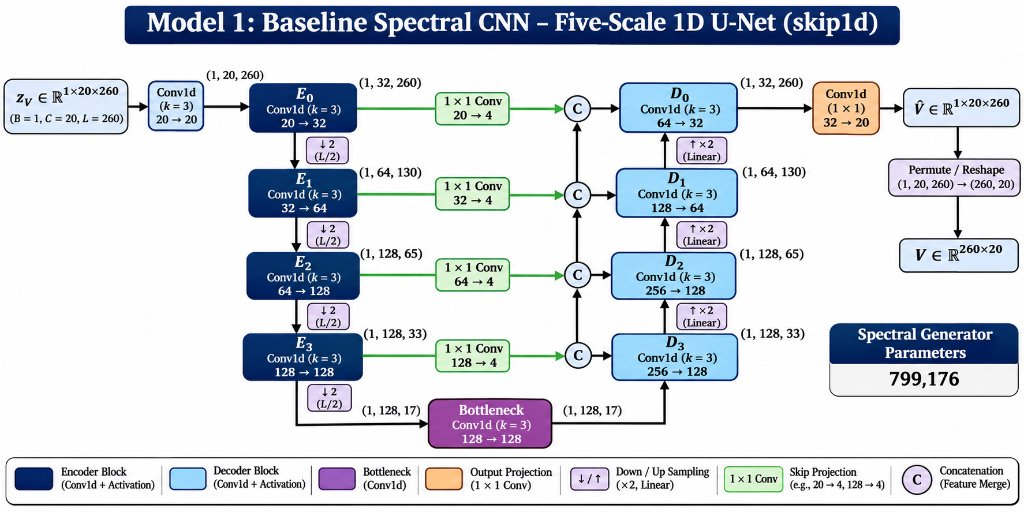
\includegraphics[width=\textwidth]{figures/architecture_model1_baseline_cnn.jpg}
    \caption{Model 1: Baseline 1D CNN Skip Network (\texttt{skip1d}).}
    \label{fig:model1_baseline}
\end{subfigure}
\hfill
\begin{subfigure}[b]{0.48\textwidth}
    \centering
    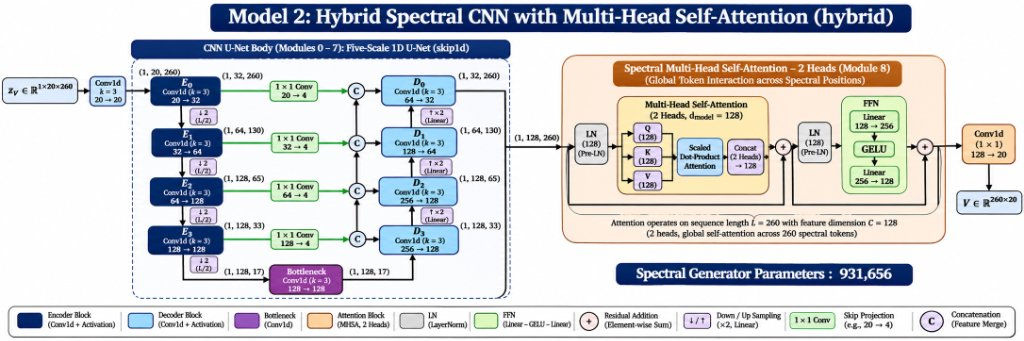
\includegraphics[width=\textwidth]{figures/architecture_model2_hybrid_attention.jpg}
    \caption{Model 2: Hybrid CNN--Attention (\texttt{hybrid}).}
    \label{fig:model2_hybrid}
\end{subfigure}

\vspace{0.2cm}
\begin{subfigure}[b]{0.48\textwidth}
    \centering
    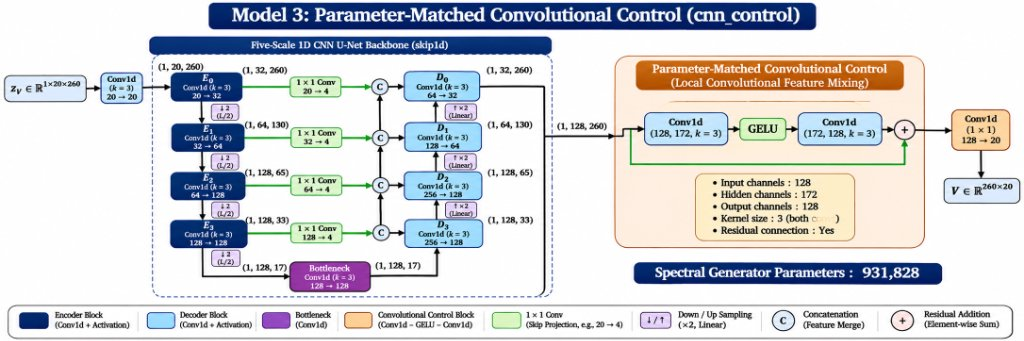
\includegraphics[width=\textwidth]{figures/architecture_model3_conv_control.jpg}
    \caption{Model 3: Conv Control (\texttt{cnn\_control}).}
    \label{fig:model3_conv_control}
\end{subfigure}
\hfill
\begin{subfigure}[b]{0.48\textwidth}
    \centering
    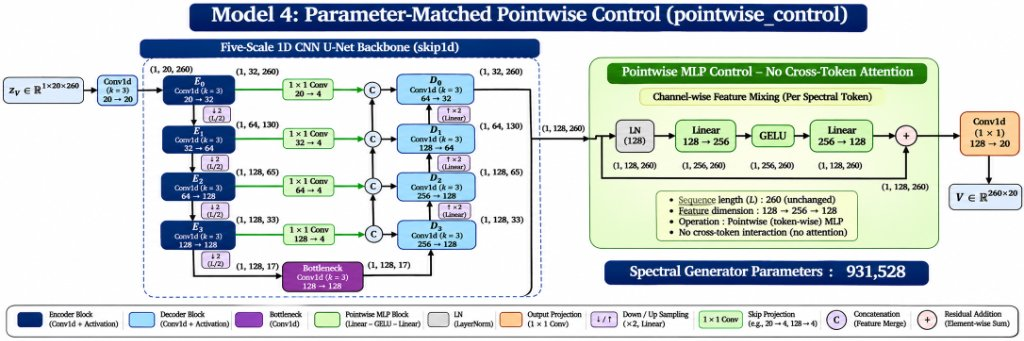
\includegraphics[width=\textwidth]{figures/architecture_model4_pointwise_control.jpg}
    \caption{Model 4: Pointwise Control (\texttt{pointwise\_control}).}
    \label{fig:model4_pointwise}
\end{subfigure}

\vspace{0.2cm}
\begin{subfigure}[b]{0.96\textwidth}
    \centering
    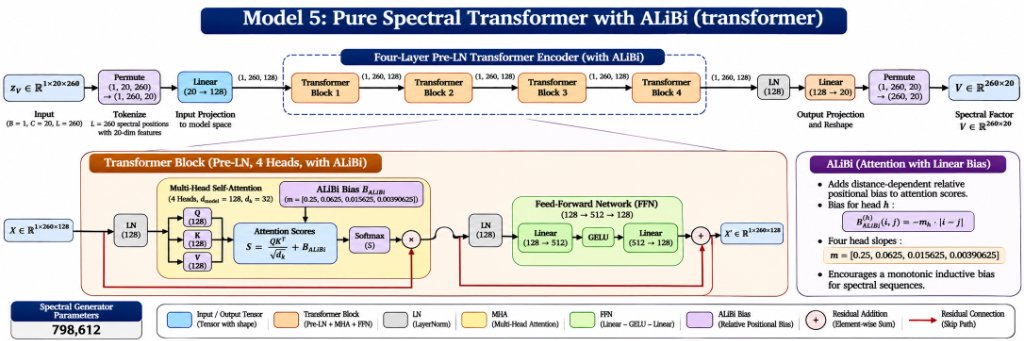
\includegraphics[width=\textwidth]{figures/architecture_model5_pure_transformer.jpg}
    \caption{Model 5: Pure Spectral Transformer with ALiBi (\texttt{transformer}).}
    \label{fig:model5_transformer}
\end{subfigure}

\caption{Detailed Architectural Schematics of the Five Investigated Spectral Factor Generator Networks ($f_V$). All architectures map latent code $\mathbf{z}_V \in \mathbb{R}^{1 \times 20 \times 260}$ to the spectral factor matrix $\mathbf{V} \in \mathbb{R}^{260 \times 20}$. (a) Baseline 5-scale 1D CNN U-Net with multi-scale skip connections, (b) Hybrid CNN with Pre-LN Multi-Head Self-Attention (2 heads), (c) Parameter-matched 1D Conv Control ($d_{\text{hid}}=172$), (d) Parameter-matched Pointwise Control ($k=1$), and (e) Pure Spectral Transformer with Attention with Linear Biases (ALiBi).}
\label{fig:architecture_pipeline}
\end{figure}

\begin{enumerate}[noitemsep, topsep=1pt]
    \item \textbf{Model 1: Baseline CNN (\texttt{skip1d}):} Standard 5-scale 1D U-Net/Skip network with $3 \times 1$ convolutions, reflection padding, LeakyReLU ($\alpha=0.2$), and multi-scale skip connections. Sequence length reduces $260 \to 130 \to 65 \to 33 \to 17$ and reconstructs via linear upsampling. Provides strong local spectral translational equivariance. Total parameters: \textbf{3,005,328} ($799,176$ spectral).
    \item \textbf{Model 2: Hybrid CNN--Attention (\texttt{hybrid}):} Augments the U-Net body output ($L=260, d=128$) with a 2-head Pre-LN Multi-Head Self-Attention ($d_\text{model}=128, d_k=64$) module and FFN ($d_\text{ffn}=256$, GELU) across all $260$ spectral bands: $\mathbf{X}' = \mathbf{X} + \text{MHSA}(\text{LN}(\mathbf{X}))$, $\mathbf{X}_\text{out} = \mathbf{X}' + \text{FFN}(\text{LN}(\mathbf{X}'))$. Integrates global token-to-token contextual routing. Total parameters: \textbf{3,137,808} ($+132,480$ over Baseline).
    \item \textbf{Model 3: Conv Control (\texttt{cnn\_control}):} Replaces MHSA with a parameter-matched 1D conv residual block (\texttt{Conv1d(128, 172, k=3)} + \texttt{GELU} + \texttt{Conv1d(172, 128, k=3)}) followed by LayerNorm, analytically calibrated to match Model 2 capacity within $172$ parameters. Total parameters: \textbf{3,137,980}.
    \item \textbf{Model 4: Pointwise Control (\texttt{pointwise\_control}):} Replaces attention with dual $1 \times 1$ pointwise linear projection layers (\texttt{Linear(128, 256)} + \texttt{GELU} + \texttt{Linear(256, 128)}), eliminating cross-token spatial/temporal receptive fields ($k=1$). Total parameters: \textbf{3,137,680} (matches Model 2 within $128$ parameters).
    \item \textbf{Model 5: Pure Spectral Transformer (\texttt{transformer}):} Completely eliminates convolutions. Operates directly on the $L=260$ spectral sequence using linear token embedding ($20 \to 128$), 4 Pre-LN Transformer layers ($d=128, H=4, d_\text{ffn}=512$) with Attention with Linear Biases (ALiBi) geometric slopes $m_h = 2^{-8h/4} \in \{2^{-2}, 2^{-4}, 2^{-6}, 2^{-8}\}$, and linear output projection ($128 \to 20$). Total parameters: \textbf{3,004,764} (parameter-matched to Baseline within $564$ parameters).
\end{enumerate}

\begin{table}[htbp]
\centering
\caption{Detailed Parameter Breakdown for the Five Architectural Models on ICVL ($R=20, B=260$).}
\label{tab:model_parameter_breakdown}
\begin{adjustbox}{width=0.92\textwidth}
\begin{tabular}{lcccc}
\toprule
\textbf{Model Architecture} & \textbf{Spatial $f_U$ Params} & \textbf{Spectral $f_V$ Params} & \textbf{Total Params} & \textbf{Param Delta vs Baseline} \\
\midrule
\textbf{1. Baseline CNN} & $2,206,152$ & $799,176$ & $3,005,328$ & Baseline ($0$) \\
\textbf{2. Hybrid CNN--Attention} & $2,206,152$ & $931,656$ & $3,137,808$ & $+132,480$ ($+4.4\%$) \\
\textbf{3. Conv Control} & $2,206,152$ & $931,828$ & $3,137,980$ & $+132,652$ ($+4.4\%$) \\
\textbf{4. Pointwise Control} & $2,206,152$ & $931,528$ & $3,137,680$ & $+132,352$ ($+4.4\%$) \\
\textbf{5. Spectral Transformer} & $2,206,152$ & $798,612$ & $3,004,764$ & $-564$ ($-0.02\%$) \\
\bottomrule
\end{tabular}
\end{adjustbox}
\end{table}

\subsection{Methodology for the Nine Research Extensions}
\label{subsec:extensions_methodology}

\textbf{Extension 1: Self-Supervised Adaptive Rank Selection:} DeepTensor assumes a fixed rank $R$. We formulate a bottom-up rank growth algorithm starting from $R_\text{active} = 4$ ($R_\text{max} = 30$). Every $\Delta E = 200$ epochs, validation loss change $\Delta \mathcal{L}_\text{val} = (\mathcal{L}_\text{val}^{(t-\Delta E)} - \mathcal{L}_\text{val}^{(t)}) / \mathcal{L}_\text{val}^{(t-\Delta E)}$ is audited. If $\Delta \mathcal{L}_\text{val} < \epsilon_\text{plateau} = 0.005$ and $R_\text{active} < R_\text{max}$, rank expands by $\Delta R = 2$ with smooth random initialization.

\textbf{Extension 2: Factor Group-Sparsity (Group Lasso) Regularization:} To test top-down pruning from $R_\text{max} = 30$, we apply a joint Group Lasso penalty across unnormalized factor columns:
\begin{equation}
\label{eq:group_lasso}
\mathcal{R}(\mathbf{U}, \mathbf{V}) = \sum_{r=1}^{R_\text{max}} \sqrt{\|\mathbf{u}_r\|_2^2 + \|\mathbf{v}_r\|_2^2}, \qquad \mathcal{L}_\text{total} = \mathcal{L}_\text{train} + \lambda \cdot \mathcal{R}(\mathbf{U}, \mathbf{V})
\end{equation}
evaluated across $\lambda \in \{0.0, 10^{-4}, 10^{-3}, 10^{-2}\}$. Component power is measured as $\text{power}_r = \|\mathbf{u}_r\|_2 \cdot \|\mathbf{v}_r\|_2$.

\textbf{Extension 3: Mask-Aware Tensor Completion:} Given observation mask $\mathbf{M} \in \{0, 1\}^{H \times W \times B}$ with missingness ratios $p \in \{0.20, 0.50, 0.80\}$, we optimize the masked reconstruction loss:
\begin{equation}
\label{eq:masked_loss}
\mathcal{L}_\text{mask}(\boldsymbol{\theta}) = \frac{\sum_{h, w, b} M_\text{train}(h, w, b) \cdot |\hat{Y}(h, w, b) - Y^\text{noisy}(h, w, b)|}{\sum_{h, w, b} M_\text{train}(h, w, b)}
\end{equation}
Missing voxels receive zero backpropagation gradient, testing self-supervised imputation on unobserved entries.

\textbf{Extension 4: Noise-Type Robustness at Matched Input Corruption:} We isolate three noise regimes: (a) Pure Gaussian ($\mathcal{N}(0, \sigma^2)$); (b) Pure Poisson ($\mathcal{P}(X \tau)/\tau$); and (c) Mixed Poisson--Gaussian. Parameters are calibrated to ensure identical input corruption ($\text{PSNR}_\text{input} \approx 28.43\text{ dB}$).

\textbf{Extension 5: Empirical Ensemble Disagreement as Uncertainty Proxy:} An ensemble of $N=5$ models with distinct seeds ($s \in \{101, \dots, 105\}$) is trained on identical data. Empirical disagreement is the sample variance: $\sigma_\text{disagreement}^2(h, w, b) = \frac{1}{N-1} \sum_{n=1}^N (\hat{Y}^{(n)}(h, w, b) - \bar{Y}(h, w, b))^2$. We evaluate Pearson $r$, Spearman $r_s$, and partial correlation controlling for image edge gradient $\|\nabla Y^\text{clean}\|$.

\textbf{Extension 6: Computational Efficiency Analysis:} Designated as \textit{Planned / Deferred} in project execution to prioritize Extensions 7--9. Baseline execution is audited at $30.4\text{ ms}$/epoch with peak VRAM of $642.9\text{ MB}$.

\textbf{Extension 7: Factor Interpretability and Progressive Ablation:} Extracted factor matrices $\mathbf{U} \in \mathbb{R}^{HW \times 20}$ and $\mathbf{V} \in \mathbb{R}^{B \times 20}$ are ordered by Frobenius energy $E_r = \|\mathbf{u}_r\|_F \cdot \|\mathbf{v}_r\|_F$. Progressive top-$k$ reconstructions determine empirical threshold $k^*$ achieving within $0.1\text{ dB}$ of full $R=20$ quality. Factor orthogonality is evaluated via pairwise cosine similarities.

\textbf{Extensions 8 \& 9: Hybrid Attention and Pure Spectral Transformer:} Evaluates 4-head MHSA at the spectral CNN bottleneck (Ext 8) and a 4-layer Pre-LN Spectral Transformer with ALiBi relative biases $\text{Attention}_h(\mathbf{Q}, \mathbf{K}, \mathbf{V}_\text{val}) = \text{softmax}(\frac{\mathbf{Q}_h \mathbf{K}_h^T}{\sqrt{d_k}} - m_h \cdot |i - j|) \mathbf{V}_\text{val}$ with $m_h = 2^{-8h/H}$ (Ext 9), benchmarked against parameter-matched convolutional and pointwise controls.
